
\section{Evaluation}
\label{sec-evaluation}
We evaluate 20 aligned, instruction-following models from Anthropic, OpenAI, Google, Cohere, Gemma~2, and Llama~3 (Table~\ref{tab:models}).
Where applicable, we disable retrieval-augmented generation and tool-use.
We independently sample 10 generations with temperature $1.0$---a best-case setting for diversity, as most APIs default to lower temperatures or nucleus sampling.

\obtodo[id=nb-eval-20, created=2025-02-21T08:30:00.000Z, updated=2025-03-18T09:11:00.000Z, completed=2025-03-18T09:11:00.000Z]{Run k=10, T=1 inference, partition, and score for all 20 models on NB-Curated and NB-WildChat.}

\begin{table}[t]
\centering
\small
\caption{Models used as baselines, with mean $\mathrm{distinct}_{10}$ and $\mathrm{utility}_{10}$ over 10 generations.}
\label{tab:models}
\begin{tabular}{llcc}
\toprule
Provider & Variant & Distinct$_{10}$ & Utility$_{10}$ \\
\midrule
Anthropic & Claude-3.5 Haiku & 1.94 & 2.50 \\
 & Claude-3.5 Sonnet & 1.76 & 2.36 \\
 & Claude-3 Opus & 2.04 & 2.67 \\
OpenAI & gpt-4o-mini & 2.65 & 3.11 \\
 & gpt-4o & 2.88 & 3.27 \\
Gemini & gemini-1.5-pro & 1.85 & 2.73 \\
 & gemini-2.0-flash-lite & 2.83 & 3.20 \\
 & gemini-2.0-flash & 2.81 & 3.17 \\
 & gemini-2.0-pro & 2.25 & 2.64 \\
Cohere & command-r7b & 3.58 & 3.35 \\
 & command-r & 2.68 & 2.98 \\
 & command-r-plus & 2.79 & 3.08 \\
Gemma 2 & gemma-2-2b-it & 5.66 & 4.63 \\
 & gemma-2-9b-it & 3.25 & 3.93 \\
 & gemma-2-27b-it & 3.03 & 3.77 \\
Llama 3 & Llama-3.2-1B & 6.74 & 2.81 \\
 & Llama-3.2-3B & 5.10 & 3.24 \\
 & Llama-3.1-8B & 5.24 & 3.76 \\
 & Llama-3.3-70B & 2.49 & 2.87 \\
 & Llama-3.1-405B & 3.20 & 3.39 \\
\bottomrule
\end{tabular}
\end{table}

\obcomment[kind=result]{Locked Table 1 from the March 18 summarize.py pass. Gemma-2-2B distinct10=5.66 vs Claude-3.5-Sonnet 1.76. Llama-3.2-1B is the diversity max (6.74) but utility is only 2.81 --- small models are novel and often bad.}

\subsection{State-of-the-art models struggle to generate diverse and useful outputs}

\begin{figure}[t]
\centering
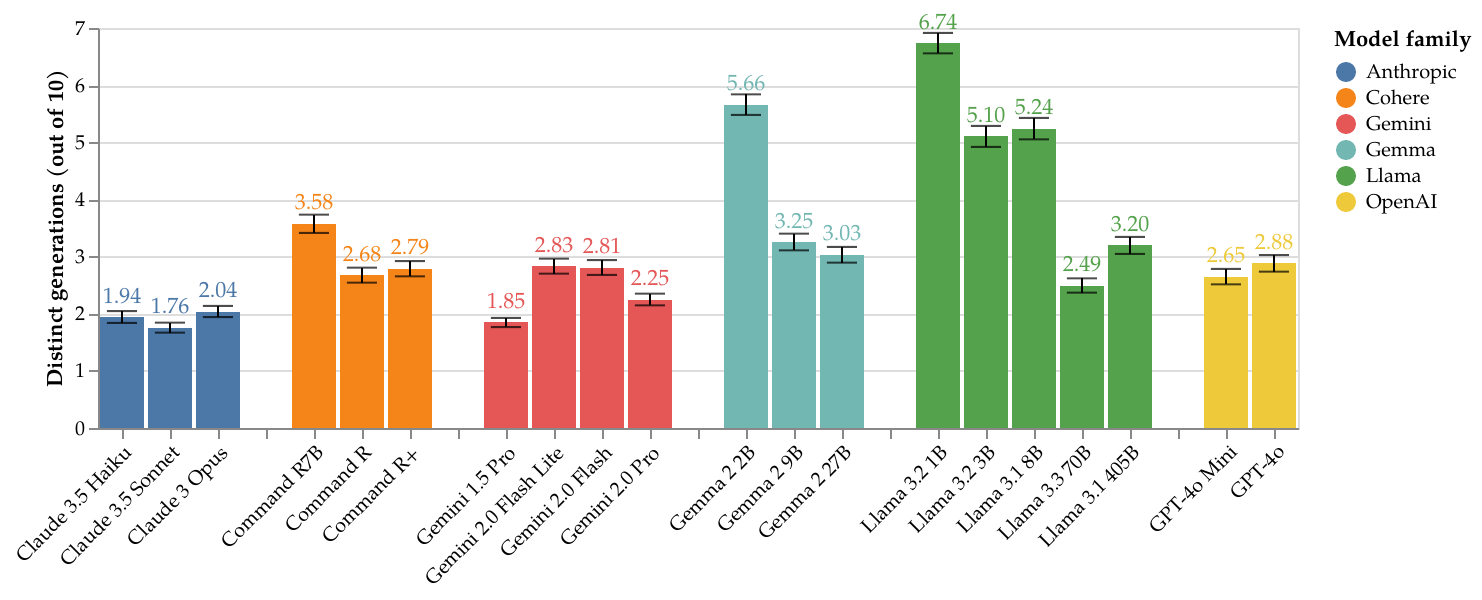
\includegraphics[width=\linewidth]{figures/distinct.png}
\caption{Average number of unique generations out of a sample of 10 for all prompts in \textsc{NoveltyBench}.
Error bars indicate 95\% confidence intervals.}
\label{fig:distinct}
\end{figure}

\begin{figure}[t]
\centering
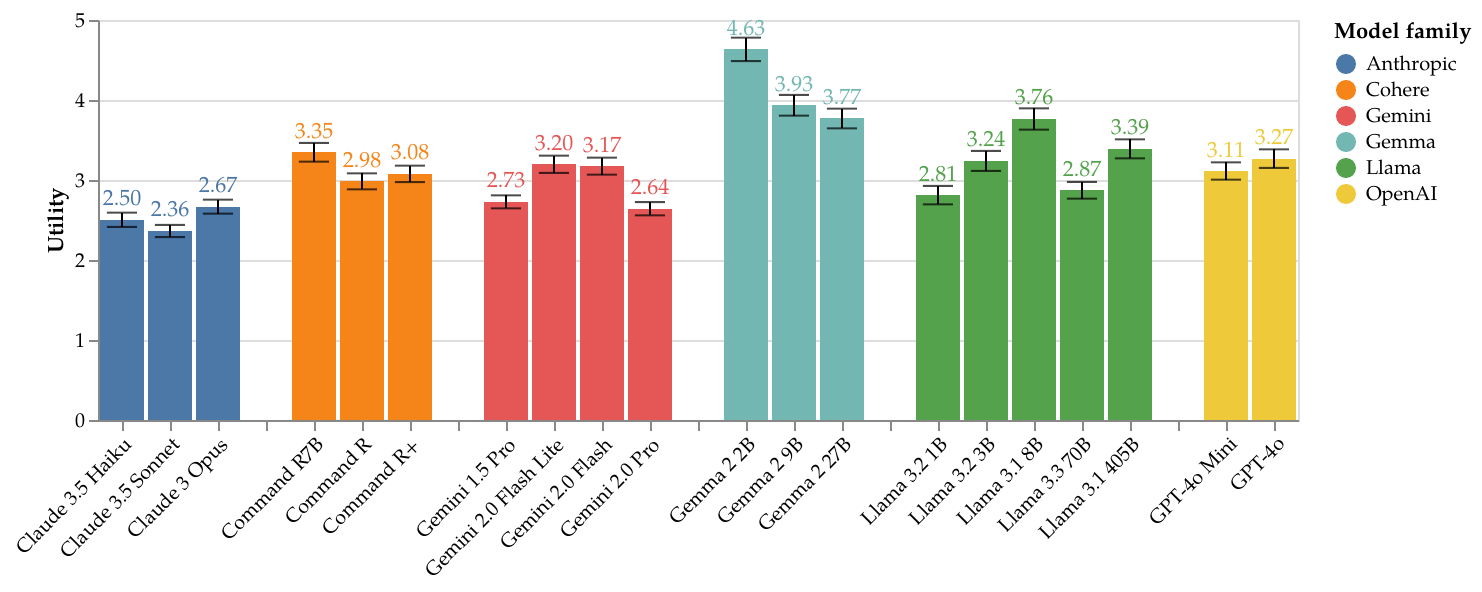
\includegraphics[width=\linewidth]{figures/utility.png}
\caption{Cumulative utility of generations of state-of-the-art models on \textsc{NoveltyBench}.
A perfectly diverse and helpful model would have cumulative utility of 10.
Error bars indicate 95\% confidence intervals.}
\label{fig:utility}
\end{figure}

Frontier models struggle to produce simultaneously diverse and useful responses.
As shown in Figure~\ref{fig:distinct}, models like Claude~3 and GPT-4o produce on average fewer than 3 distinct responses in 10 queries.
Notably, smaller models such as Gemma 2-2B and Llama 3.2-1B demonstrate the highest diversity on our benchmark.
Figure~\ref{fig:utility} further illustrates this issue by measuring cumulative utility.
Closed-source models such as Claude~3, Gemini, and GPT-4o all scored below 4 out of a maximum utility score of 10.

While larger models typically excel in standard benchmarks, they demonstrate worse diversity than smaller models in the same family.
Figure~\ref{fig:patience-comparison} shows cumulative utility as a function of patience on Gemma~2 and Llama~3, where parameter counts are public.
At patience $=0$ we are evaluating a single generation; larger models win.
As patience increases, additional novel generations are given higher weights, and larger models degrade faster because of mode collapse.

\begin{figure}[t]
\centering
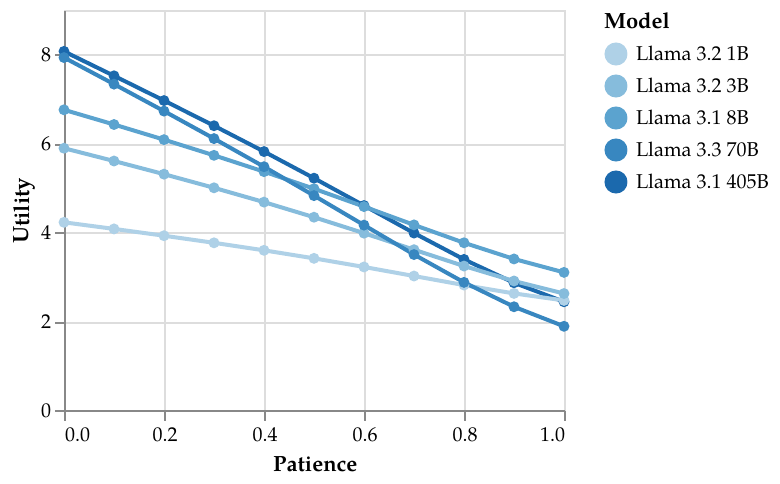
\includegraphics[width=0.49\linewidth]{figures/llama-patience.png}
\hfill
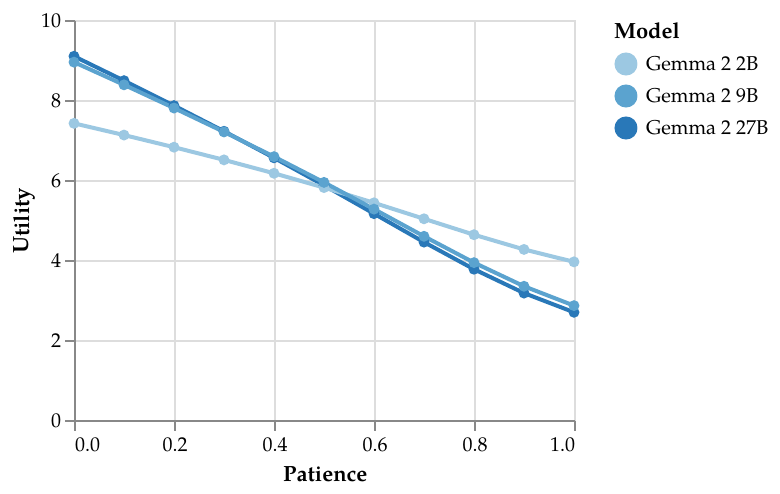
\includegraphics[width=0.49\linewidth]{figures/gemma-patience.png}
\caption{As users demand more diverse generations, models become less useful.
Larger models suffer more from degradation in utility.}
\label{fig:patience-comparison}
\end{figure}

\obclaim{Progress on single-generation benchmarks is misleading: larger models look better at $p=0$ and worse as users demand diversity.}

\subsection{Alternate prompting methods for inducing diversity}

We compare four methods on the 100 curated prompts, with eight generations to match the human pool:

\begin{itemize}
\item \textbf{Resampling:} independent samples at temperature $1.0$.
\item \textbf{Paraphrasing:} a distinct paraphrase of the original prompt for each generation.
\item \textbf{System prompt:} ``You are a producer of unique answers, and you strive to tell each user a novel answer to their question.''
\item \textbf{In-context regeneration:} after each generation, ask for a different answer while keeping previous answers in context.
\end{itemize}

\obtodo[id=nb-prompting-ablate, created=2025-03-04T12:00:00.000Z, updated=2025-03-19T20:36:14.000Z, completed=2025-03-19T20:36:14.000Z]{Ablate resampling, paraphrasing, system prompt, and in-context regeneration vs the 8-author human pool.}
\obcomment[kind=result]{Paraphrase and system prompt barely move the needle. In-context regeneration matches human distinctness; GPT-4o and Gemini 2.0 Pro even beat human utility because quality is higher. Diversity is elicit-able, not in the unconditional distribution.}

\begin{figure}[t]
\centering
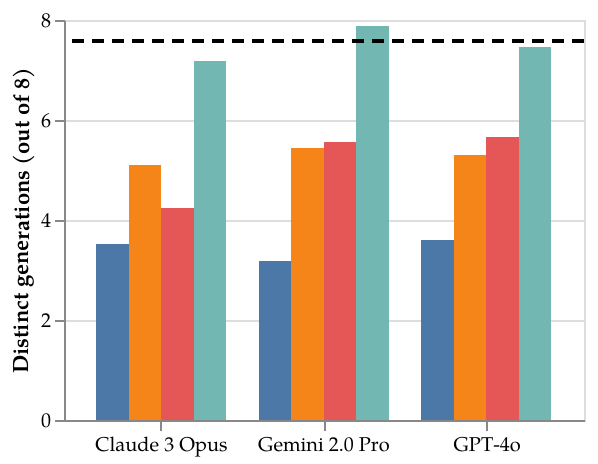
\includegraphics[width=0.49\linewidth]{figures/alternative-prompting-distinct.png}
\hfill
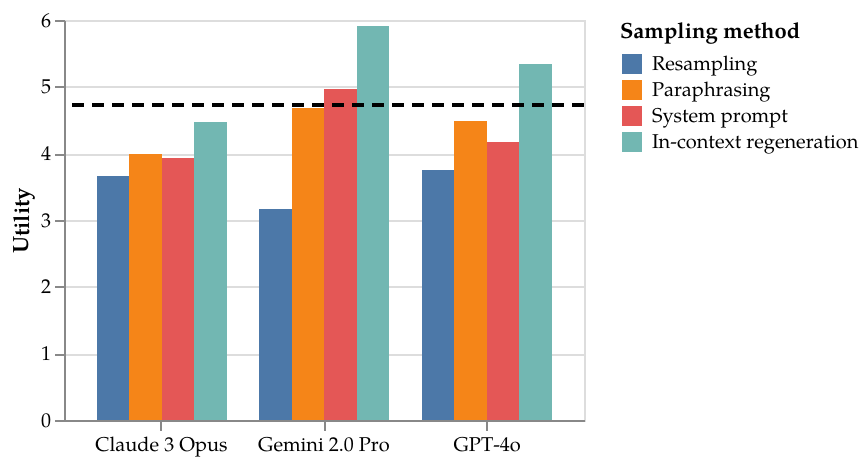
\includegraphics[width=0.49\linewidth]{figures/alternative-prompting-utility.png}
\caption{Alternative prompting methods can lead to improved novelty.
Dashed lines report diversity and utility of answers handwritten by authors.}
\label{fig:alt-prompting}
\end{figure}

As shown in Figure~\ref{fig:alt-prompting}, paraphrasing and system prompting are only marginally effective.
In-context regeneration is the most successful approach, with Claude-3 Opus, GPT-4o, and Gemini 2.0 Pro roughly matching the diversity of human writers.
Under this strategy, GPT-4o and Gemini 2.0 Pro even surpass the cumulative utility scores of human writers due to the added diversity.

Table~\ref{tab:gpt4o} shows GPT-4o collapsing under ordinary resampling: silver-mist names, Mirzakhani, and the Toyota RAV4 Hybrid recur across independent samples.

\begin{table}[t]
\centering
\scriptsize
\caption{GPT-4o responses to NB-Curated prompts under independent sampling. Bold/italics preserved from source outputs.}
\label{tab:gpt4o}
\begin{tabular}{p{0.23\linewidth}p{0.23\linewidth}p{0.23\linewidth}p{0.23\linewidth}}
\toprule
Filly name & Fields Medal & d20 & Best car 2023 \\
\midrule
Silver Mist & Maryam Mirzakhani & 14 & Toyota RAV4 Hybrid \\
``Silvermist'' & Terence Tao & 17 & Toyota RAV4 Hybrid \\
``Silvermist'' & Maryam Mirzakhani & 15 & Toyota RAV4 Hybrid \\
``Luna Cascade'' & Maryam Mirzakhani & 17 & Toyota RAV4 Hybrid \\
Luna Mist & Maryam Mirzakhani & 13 & Toyota RAV4 Hybrid \\
\bottomrule
\end{tabular}
\end{table}

\subsection{How does alignment affect diversity?}

The OLMo~2 series~\cite{olmo2025} releases weights after each post-training stage.
We evaluate 1B, 7B, 13B, and 32B after SFT, DPO, and RLVR.

\obtodo[id=nb-olmo-alignment, created=2025-03-10T09:00:00.000Z, updated=2025-03-22T15:02:47.000Z, completed=2025-03-22T15:02:47.000Z]{Evaluate OLMo 2 1B/7B/13B/32B after SFT, DPO, and RLVR on both NoveltyBench splits.}
\obcomment[kind=result]{Each alignment stage drops diversity; the steep cut is DPO. Utility still rises SFT to DPO because quality compensates. Alignment is not diversity-neutral.}

\begin{figure}[t]
\centering
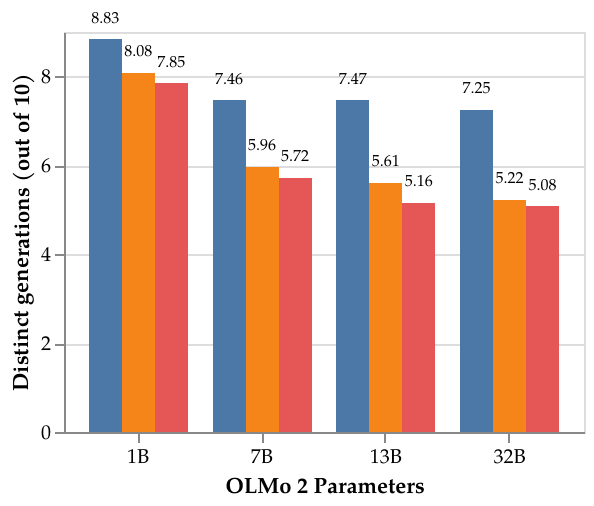
\includegraphics[width=0.49\linewidth]{figures/olmo-2_diversity_bars.png}
\hfill
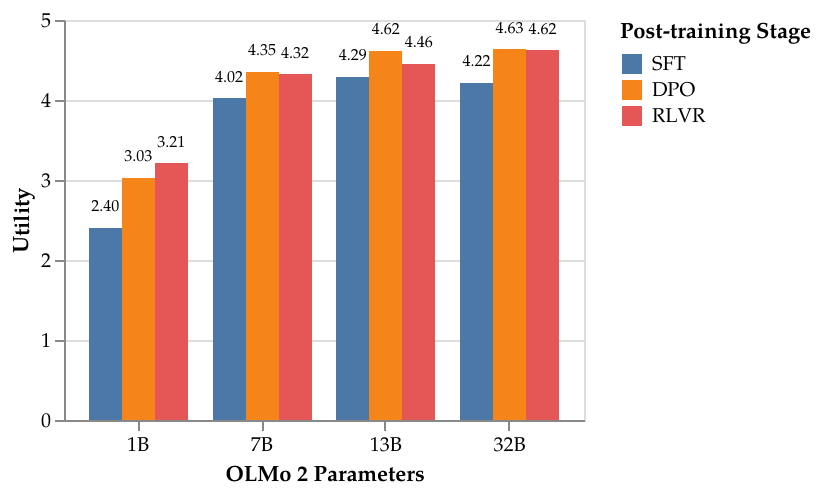
\includegraphics[width=0.49\linewidth]{figures/olmo-2_utility_bars.png}
\caption{Diversity and utility analysis of OLMo 2 models across alignment stages.}
\label{fig:olmo-analysis}
\end{figure}

Across model sizes, each alignment stage progressively reduces model diversity, with significant drops during DPO (Figure~\ref{fig:olmo-analysis}).
Quality improvements compensate: we observe utility gains when transitioning from SFT to DPO.
Alignment algorithms should be designed with output diversity in mind.
